\chapter{Diseño e implementación de los modelos o técnicas necesarias}


\section{Modelo secuencial}
En este capítulo se ah diseñado una red neuronal muy sencilla, con itención de observar los efectos que el drift puede tener en el accuracy y el loss del modelo. El esquema de la red neuronal se presenta en la tabla \ref{tab:esquemaRNN}

\begin{table}
	\centering
	\begin{tabular}{|l l l|}
		\toprule
		Model: "sequential"  & &   \\ \midrule 
		Layer (type)         &        Output Shape   &         Param  \\ \hline
		flatten (Flatten)    &        (None, 128)    &         0      \\ \hline
		dense (Dense)        &        (None, 32)     &         4128   \\ \hline
		dense\_1 (Dense)     &         (None, 32)    &         1056  \\ \hline
		dense\_2 (Dense)     &         (None, 6)     &         198   \\ \hline
		Total params: 5,382  &                       &     \\ \hline
		Trainable params: 5,382 & & \\ \hline
		Non-trainable params: 0 & & \\ \bottomrule
	\end{tabular}
\caption[Modelo de red neuronal secuencial]{Modelo de red neuronal secuencial \label{tab:esquemaRNN}}
\end{table}

\subsection{Modelo simplificado}

Primero, modelo más simple posible. Los datos de entrenamiento serán las mediciones de 1 sensor y como valores objetivo tomamos pares gases-concentración . Es decir, reducimos las mediciones a 6 parejas gas-concentración únicas tomadas por un único sensor.

Reducimos así las variables de estudio, y podemos ver el efecto del drift en las mediciones de un gas dado. Utilizando todos los datos, división entre entrenamiento y validación al 70/30, obtenemos la matriz de confusión de la Figura\ref{fig:confmatrixmodelsimple}

\begin{figure}
	\centering
	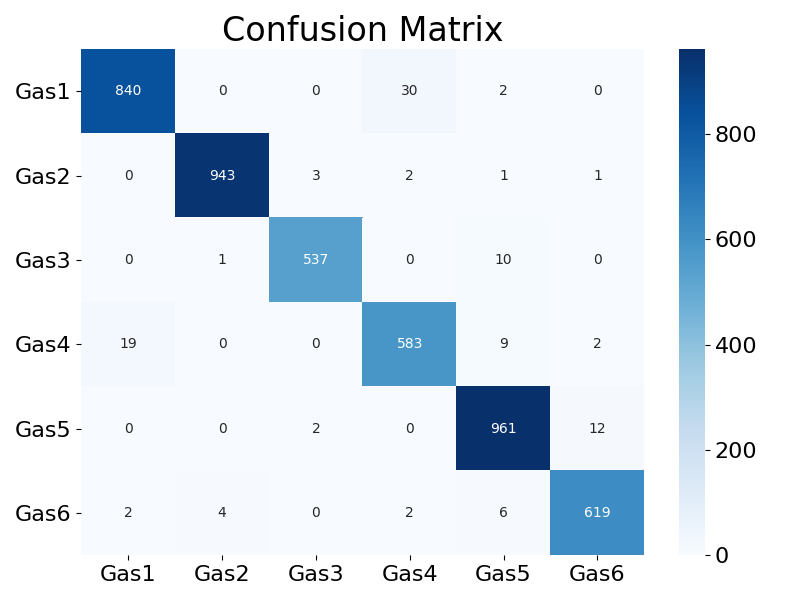
\includegraphics[width=0.7\linewidth]{../py_imgs/ConfMatrix_ModelSimple}
	\caption{Matriz de confusión del modelo utilizando todas las mediciones, entrenando al 70/30. Muy buenos resultados.}
	\label{fig:confmatrixmodelsimple}
\end{figure}

Sabemos que nuestro modelo a podido aprender a diferenciar entre los gases, pero no es realmente útil, ya que el modelo está aprendiendo cómo es un gas tanto en el primer mes de mediciones como en el último. Es decir, este modelo daría malos resultados si probamos con nuevas mediciones.

\subsection{Modelo completo}


Si este mismo modelo lo entrenamos con todos los datos disponibles de los sensores, el primer batch, y medimos el accuracy y el loss frente a los siguientes batch, obtenemos las Figuras\ref{fig:EvoModelSimpleBatch}. Se observa claramente cómo tanto el accuracy decae conformo intentamos predecir valores más lejanos. 

\begin{figure}
	\centering
	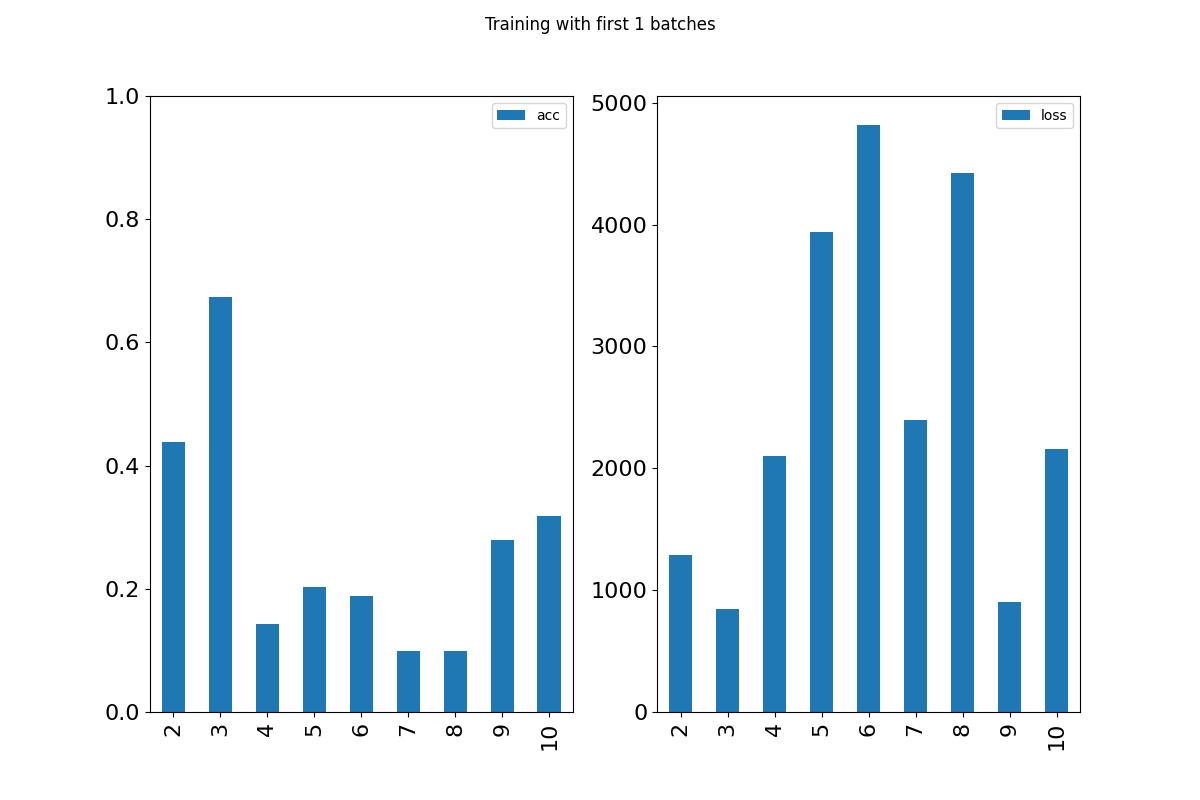
\includegraphics[width=0.45\linewidth]{../py_imgs/Step1_NBATCH_1_acc_loss}
	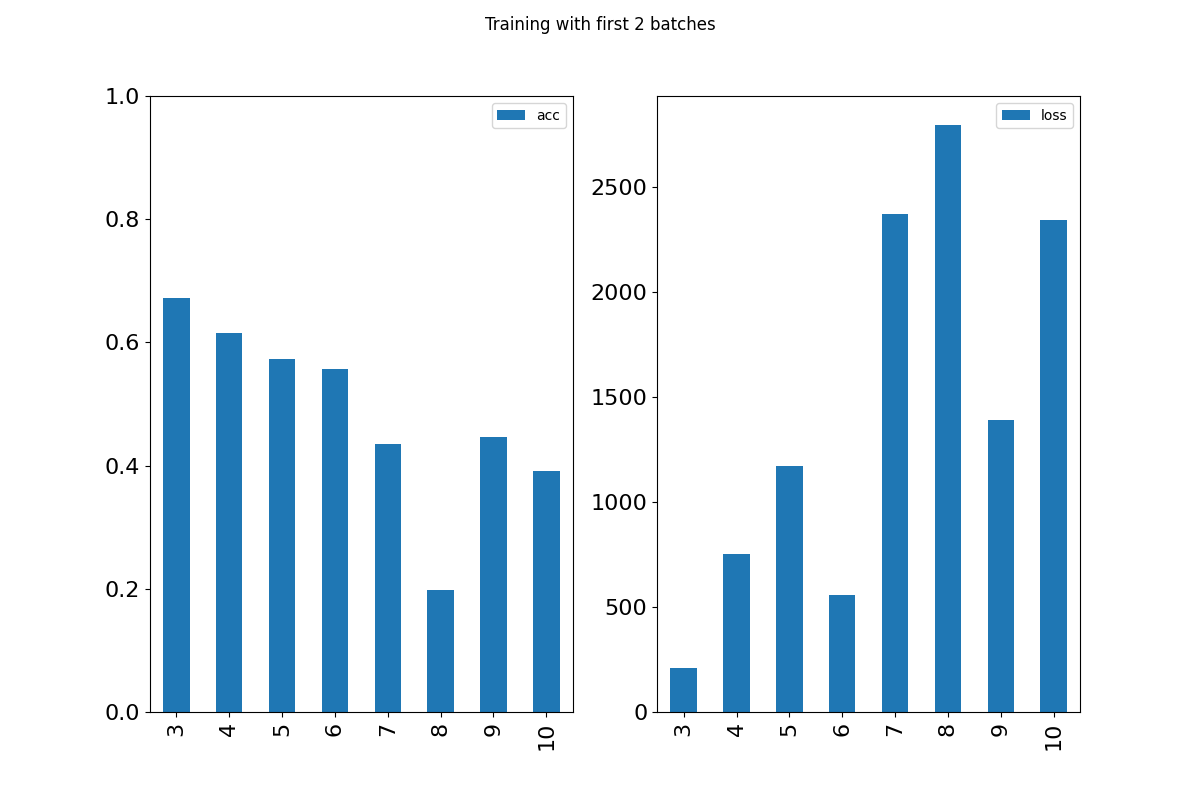
\includegraphics[width=0.45\linewidth]{../py_imgs/Step1_NBATCH_2_acc_loss}
	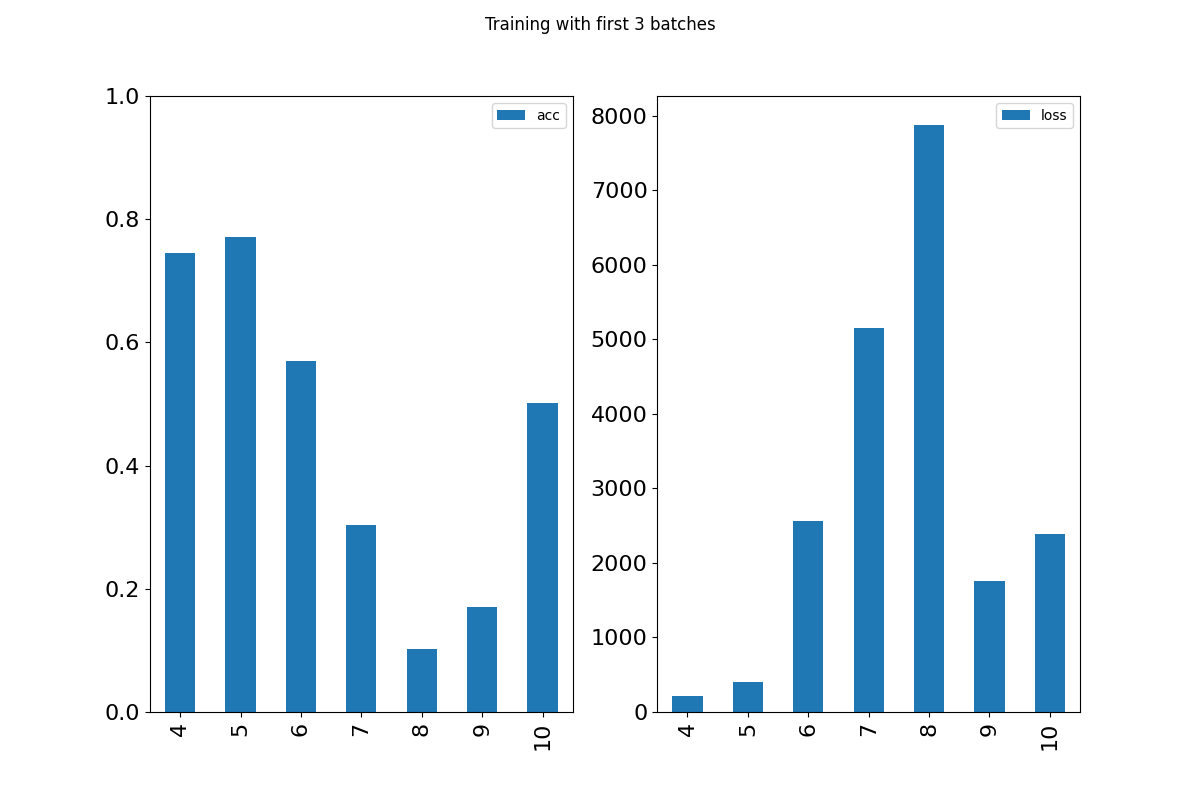
\includegraphics[width=0.45\linewidth]{../py_imgs/Step1_NBATCH_3_acc_loss}
	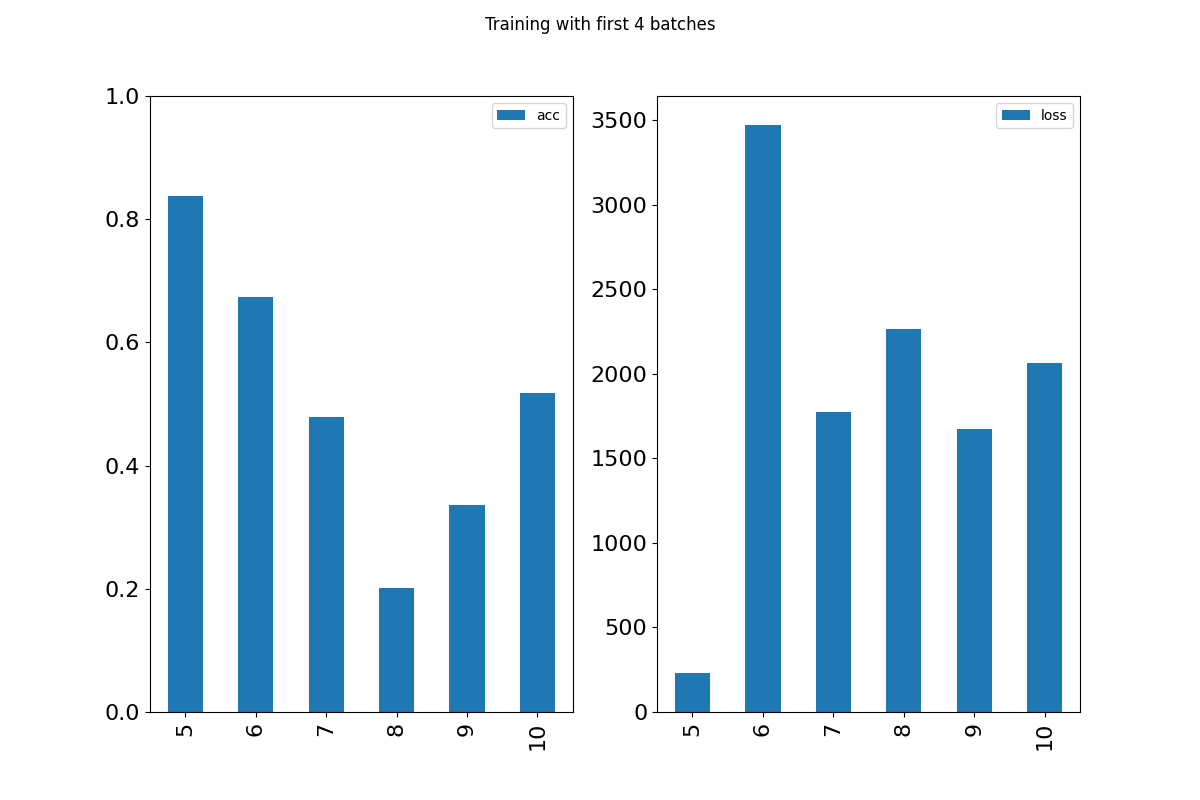
\includegraphics[width=0.45\linewidth]{../py_imgs/Step1_NBATCH_4_acc_loss}
	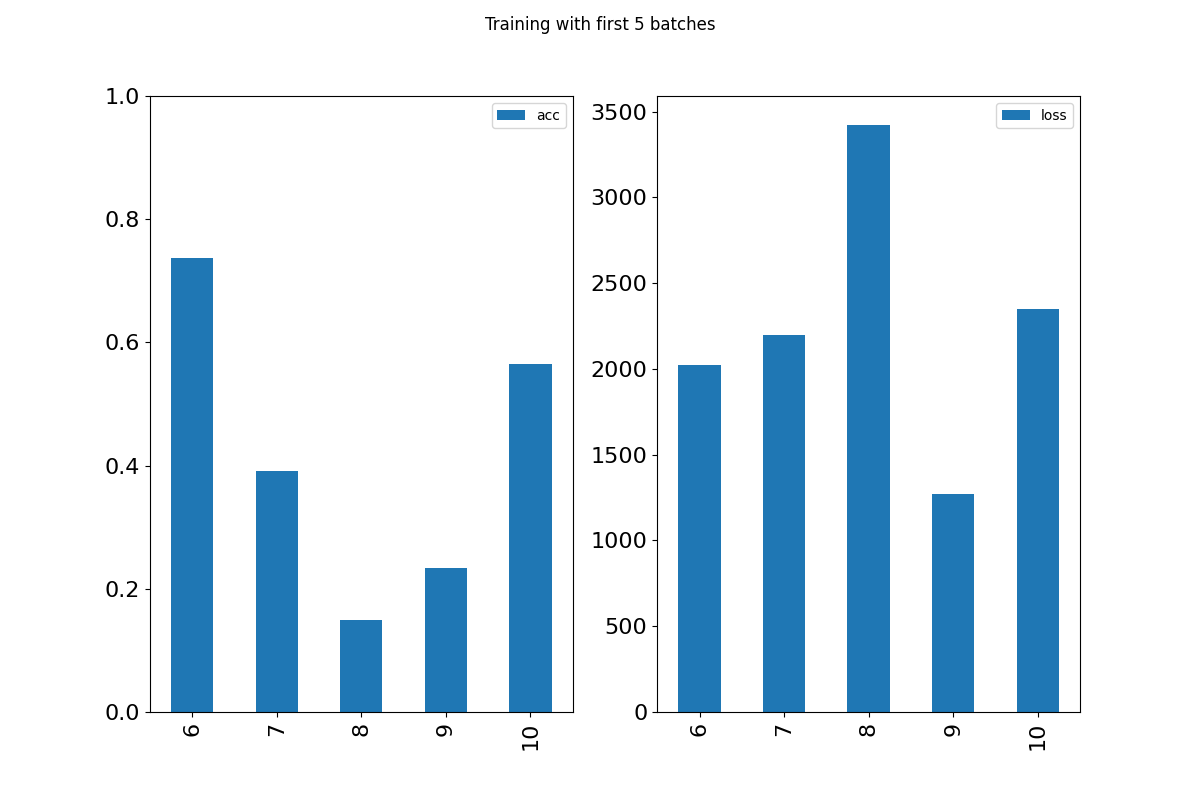
\includegraphics[width=0.45\linewidth]{../py_imgs/Step1_NBATCH_5_acc_loss}
	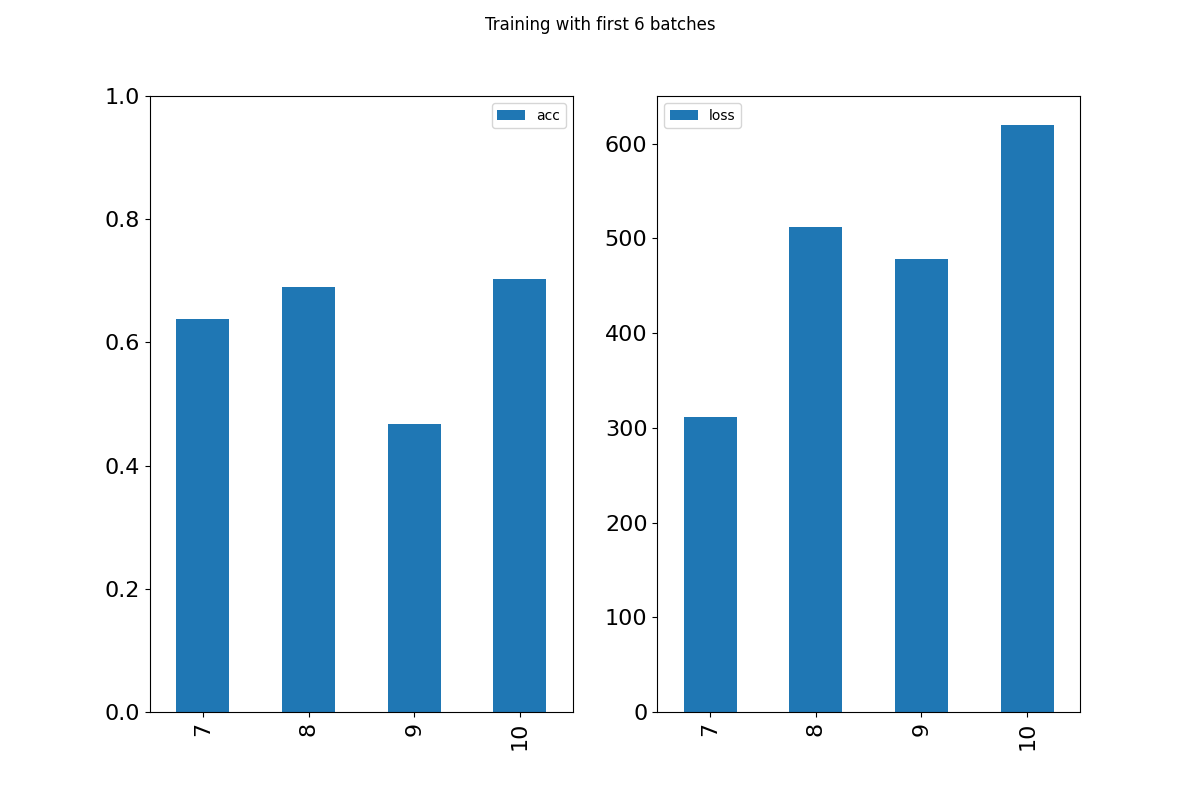
\includegraphics[width=0.45\linewidth]{../py_imgs/Step1_NBATCH_6_acc_loss}
	\caption[Evolución del drift con los resultados de validación]{Evolución del drift con los resultados de validación. Utilizando un numero N de lotes como entrenamiento, y calculando su accuracy y loss frente a los siguientes batchs de forma individual. }
	\label{fig:EvoModelSimpleBatch}
\end{figure}


Esto nos indica que la deriva es acumulativa, conforme mas nos alejamos de los meses de entrenamiento peor accuracy tiene el modelo.


Debemos mencionar que estos resultados se han obtenido utilizando los datos de los 16 sensores, que como ya se mencionó guardan una fuerte correlación. 


Esto podría hacer que el modelo no diera importancia al resto de variables, ya que siempre es necesario entrenar los modelos con variables independientes. La multicolinealidad reduce la precisión de los coeficientes de estimación, lo que debilitaría los modelos de regresión, y por tanto cualquier modelo basado en regresión: redes neuronales, random forest, etc.

Sin embargo, es posible que este efecto se vea compensado por la información añadida que sí que aporta, ya que el gas a una concentración dada pasaría de estar definido por 8 variables a 128.

Al utilizar RandomForest y LightGBM se han encontrado la misma evolución. Cabe destacar que LightGBM es increíblemente rápido para entrenar. 

\begin{figure}
	\centering
	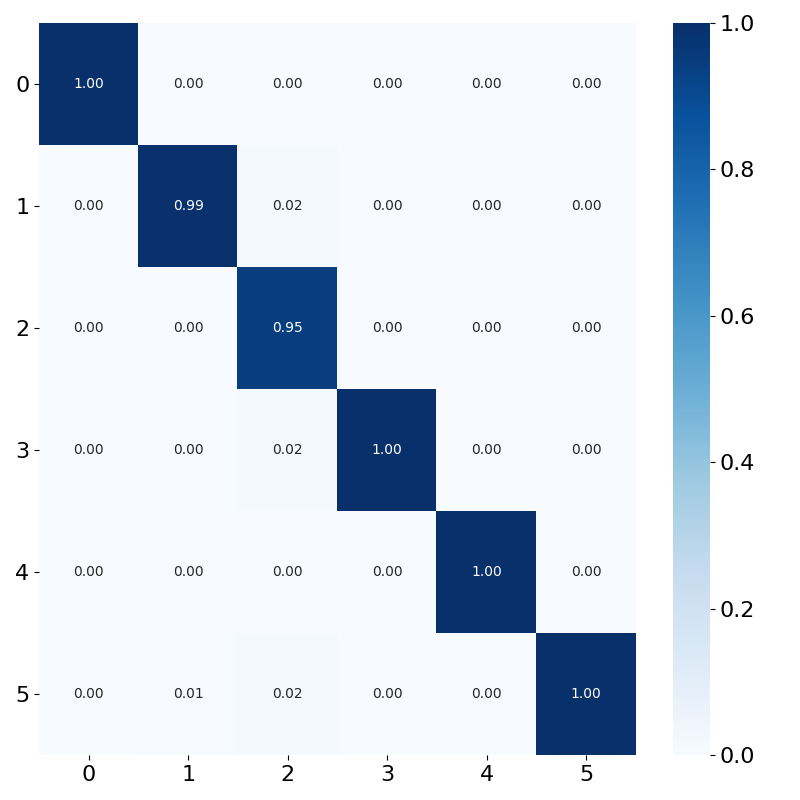
\includegraphics[width=0.6\linewidth]{../py_imgs/Setp4_conf_matrix_batch1to9}
	\caption{Matriz de confusión utlizando todos los datos disponibles de los batchs 1 a 9. Los datos de entramiento y datos de validacion se han divido al 70-30}
	\label{fig:setp4confmatrixbatch1to9}
\end{figure}

\begin{figure}
	\centering
	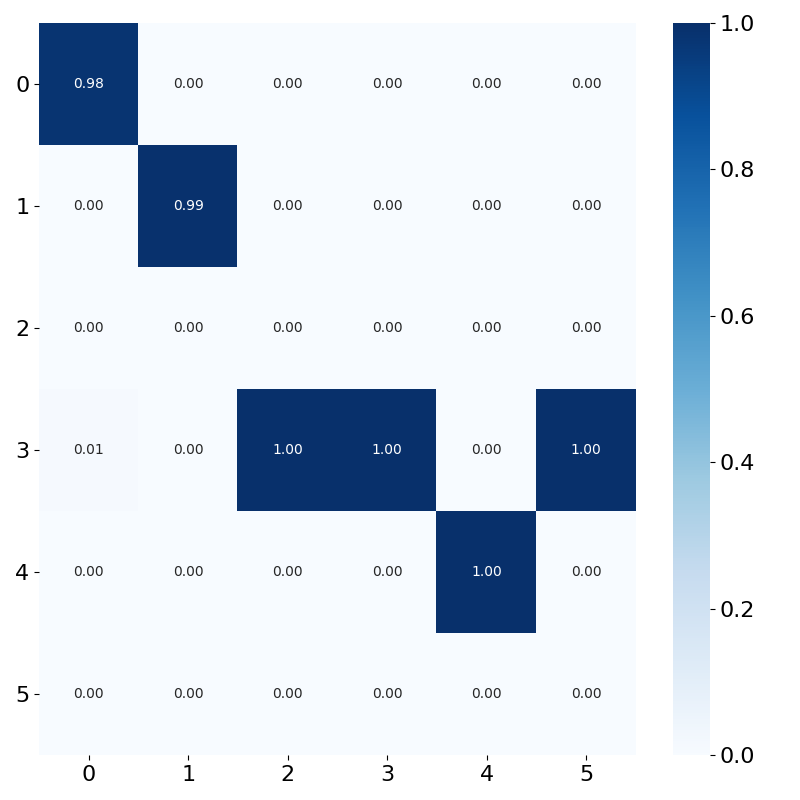
\includegraphics[width=0.6\linewidth]{../py_imgs/Setp4_conf_matrix_test_with_batch10}
	\caption{Matriz de confusión enfrentando el modelo a los datos nuevos proporcionados en le batch 10. El modelo sigue siendo preciso, pero no accurate, ya que confunde los gases.Podemos ver que 2 y 5 son catalogados como gas3. }
	\label{fig:setp4confmatrixbatch1to9}
\end{figure}


\subsection{Efecto del tipo de sensor}

Vamos a entrenar 4 modelos, uno utilizando las mediciones de cada tipo de sensor, y compararemos las matrices de confusión, para ver si hay sensores que no consiguen detectar un gas específico. Denominemos al tipo de sensor A,B,C y D.

\begin{figure}
	\centering
	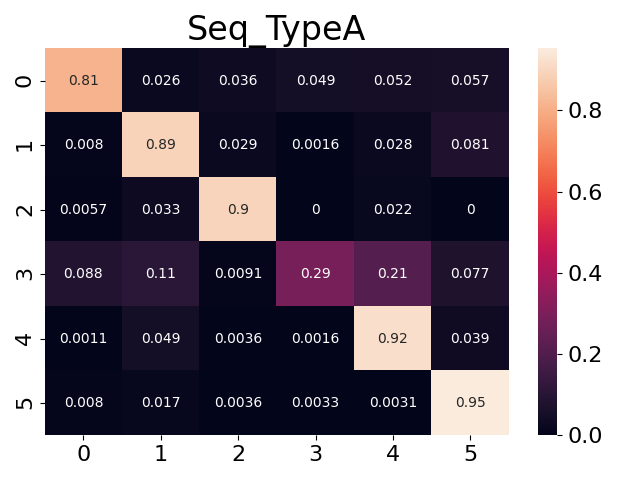
\includegraphics[width=0.45\linewidth]{../py_imgs/Conf_Seq_TypeA}
	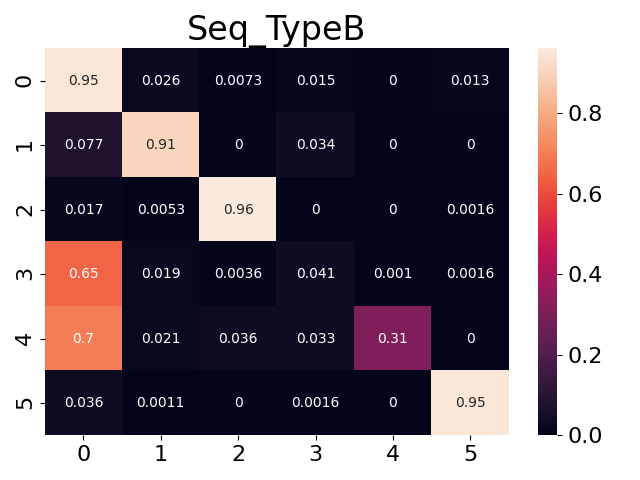
\includegraphics[width=0.45\linewidth]{../py_imgs/Conf_Seq_TypeB}
	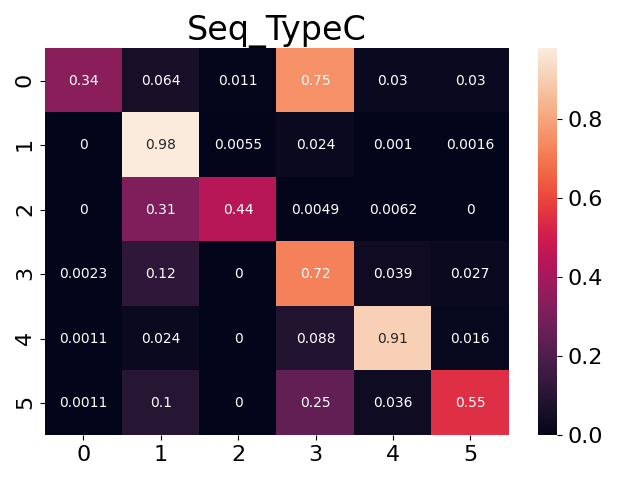
\includegraphics[width=0.45\linewidth]{../py_imgs/Conf_Seq_TypeC}
	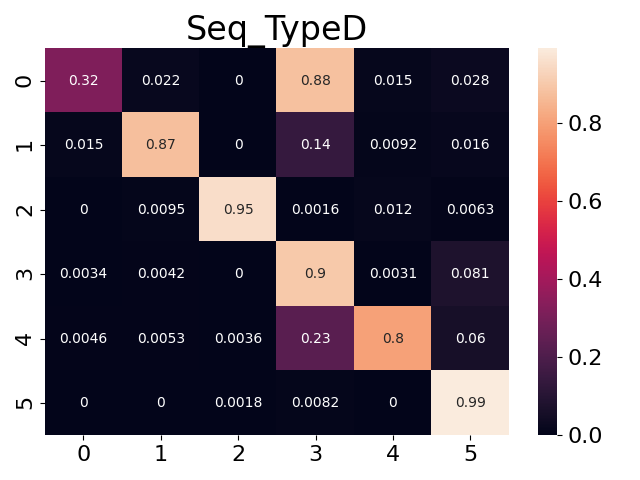
\includegraphics[width=0.45\linewidth]{../py_imgs/Conf_Seq_TypeD}
	\caption[Matrix de confusión para cada tipología de sensor]{ Matriz de confusión utilizando solo sensores tipo A en la img sup izq, solo sensores tipo B en la img sup drech y así sucesivamente. El sensor tipo A predice bastante bien todos los tipos de gases, los sensores B no consiguen detectar dos gases, y los tipo C y D fallan mucho al detectar un gas en concreto.   }
	\label{fig:confseqtypea}
\end{figure}

\begin{figure}
	\centering
	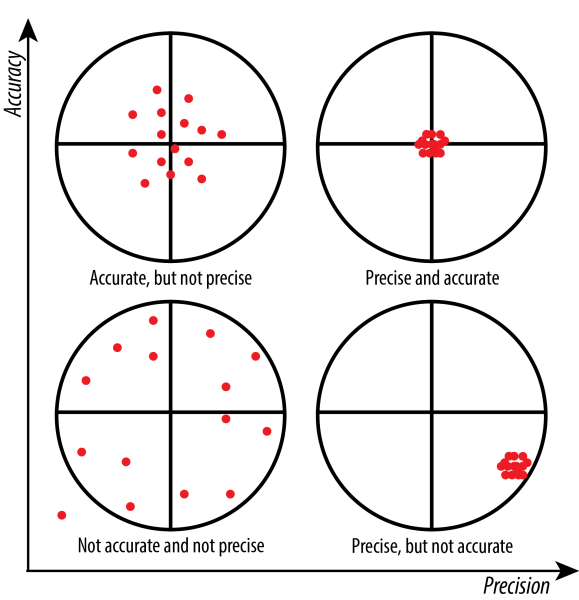
\includegraphics[width=0.7\linewidth]{../py_imgs/precsion_vs_accuracy}
	\caption[Accuracy y precision]{Es importante diferenciar entre accuracy y precision, ya que según de que forma fallen nuestros modelos, ya que podria aportarnos información sobre el problema al que nos enfrentamos.}
	\label{fig:precisionvsaccuracy}
\end{figure}

Las diferencias de sensibilidad entre cada sensor del mismo tipo influyen en sus predicciones. La efectividad de los modelos basados en cada sensor es peor que el modelo total. Pero cabe la posibilidad de que el modelo de 128 dimensiones esté desechando muchas dimensiones, no utilizando la información proporcionada por todos los sensores.

La Figura \ref{fig:confseqtypea} nos da mucha informacón sobre qué está ocurriendo , ya que el modelo de tipoB no es accuracy, pero sí precise, ya que los gases 3, y 4 los está clasificando como gas0. (ver Figura \ref{fig:precisionvsaccuracy})

Si utilizamos RandomForest o LightGBM, podemos representar los shap values, y ver cuales son las variables que más están influyendo en el resultado de la predicción. Los shap values para un modelo entrenado únicamente con un sensor son razonables, \ref{fig:step4lgbmonesensor}, pero si utilizamos las 128 componentes disponibles vemos que el modelo está desechando mucha información, Figura \ref{fig:step4lgbmall-data}

\begin{figure}
	\centering
	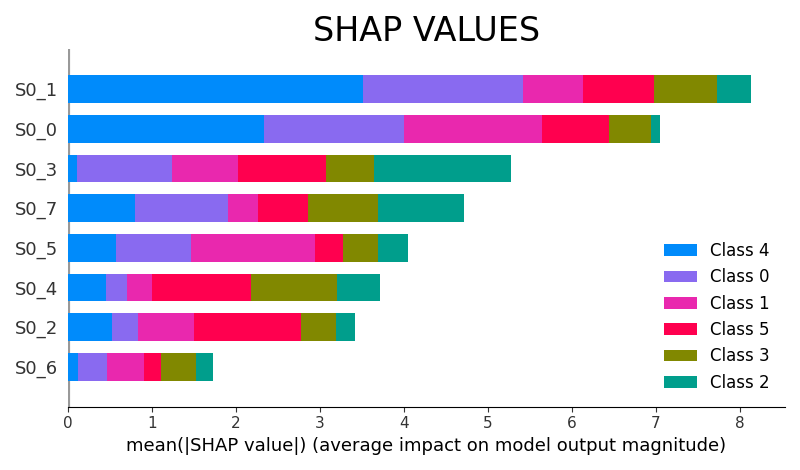
\includegraphics[width=0.7\linewidth]{../py_imgs/Step4_LGBM_one_sensor}
	\caption[Modelo LGBM-1sensor]{Modelo de LGBM para un sensor. Prácticamente todas las variables tienen influencia en la predicción. }
	\label{fig:step4lgbmonesensor}
\end{figure}

\begin{figure}
	\centering
	\includegraphics[width=0.7\linewidth]{"../py_imgs/Step4_LGBM_all data"}
	\caption[Modelo LGBM-6sensores]{Modelo de LGBM para todos los sensores. podemos obtervar que está tomando compoenntes aleatorias de cada sensor. De las 128 componentes, podriamos quedarnos únicamente con las 20 primeras y los resultados de la predicción serían similares. }
	\label{fig:step4lgbmall-data}
\end{figure}


\section{Algoritmos no supervisados}

Para este apartado se ha elegido dos algoritmos de clasificación no supervisada, KMeans clustering y TSNE. 

Para el algotirmo de KMeans clustering se ha realizado la Figura \ref{fig:step03color-for-each-cluster}. En la imagen derecha se puede apreciar cómo hay mediciones que están bien diferenciadas del resto, mientras que hay un gran conjunto de ellas que el algoritmo no ha podido separarlas, ya que se trata de mediciones muy similares, pero sin embargo e trata de gases distintos. 
	
Esto pone de manifiesto la complejidad del problema, ya que si las señales para cada gas fueran suficientemente diferentes entre sí, el algoritmo de clustering no habría encontrado problema en diferenciarlas. 

\begin{figure}[h!]
	\centering
	\includegraphics[width=0.45\linewidth]{"../py_imgs/Step0_3_Color for each cluster_3d_All data"}
	\includegraphics[width=0.45\linewidth]{"../py_imgs/Step0_3_Color for each gas_3d_All data"}
	\caption[Resultados KMeans Clustering]{En ambas imagenes los puntos están distribuidos según los planos propuestos por PCA. En la imagen a la izq podemos ver los grupos propuestos por el algorimo de KMeans Clusteing, mientras que a la derecha se ha coloreado cada punto según a qué gas pertenece dicha medición. }
	\label{fig:step03color-for-each-cluster}
\end{figure}


El algoritmo de clasificación no supervisada TSNE \emph{t-distributed stochastic neighbor embedding}, nos ha dado como resultado la Figura \ref{fig:step03tsnecolor-for-each-gas}, donde se ha coloreado cada punto en función del gas al que pertenece. Esta imagen pone de manifiesto cómo hay mediciones que a pesar de pertenecer a otros gases, son tan similares a otras que acaban en un clúster que no les correponde. 

\begin{figure}[h!]
	\centering
	\includegraphics[width=0.9\linewidth]{"../py_imgs/Step0_3_TSNE_3d_All data"}
	\caption[Resultados TSNE]{Resultados TSNE. Se han coloreado los  puntos según a qué gas pertenece. Se observa que no es capaz de separar los clusters de forma unívoca para cada medición.}
	\label{fig:step03tsnecolor-for-each-gas}
\end{figure}

Si reducimos la dificultad del problema, creando un dataset con las mediciones de un solo sensor, concentraciones por debajo de 100, y utilizando el primer batch, obtenemos los gráficos de las Figuras \ref{fig:step03kmeans-reduced-color-for-each-gas}

\begin{figure}[h!]
	\centering
	\includegraphics[width=0.45\linewidth]{"../py_imgs/Step0_3_Color for each gas_Batch1_Sensor1_Conc less 100ppmv"}
	\includegraphics[width=0.45\linewidth]{"../py_imgs/Step0_3_Color for each gas_3d_Batch1_Sensor1_Conc less 100ppmv"}
	\caption[Resultados PCA modelo simplificado]{Resultados PCA para los datos del batch 1, sensor1 y concentraciones por debajo de 100ppmv. Se han coloreado los  puntos según a qué gas pertenece. A la izq se ha reducido la dimensionalidad a 2d, y a la drecha a 3d. Los fases aparecen en clusters bien diferenciados}
	\label{fig:step03kmeans-reduced-color-for-each-gas}
\end{figure}

Sin embargo, si creamos un dataset que contenga las mediciones realizadas en el primer batch y en el último, y realizamos sobre éste la misma descomposición con KMeans Clustering, obtenemos la Figura \ref{fig:step03kmeans-1-10-color-for-each-gas}. En esta imagen podemos ver quie existen los mismos puntos que en la imagen anterior, pero que ha aparecido otro gruupo, otra rama, que es completamente diferente. El algoritmo de clustering nos está diciendo que los puntos del último batch no son similares a los del primero. 

\begin{figure}[h!]
	\centering
	\includegraphics[width=0.45\linewidth]{"../py_imgs/Step0_3_Color for each gas_Batch1and10_Sensor1_Conc less 100ppmv"}
	\includegraphics[width=0.45\linewidth]{"../py_imgs/Step0_3_Color for each gas_3d_Batch1and10_Sensor1_Conc less 100ppmv"}
	\caption[Resultados PCA modelo batch 1 y 10]{Resultados PCA para los datos del batch 1 y 10, sensor1 y concentraciones por debajo de 100ppmv. Se han coloreado los  puntos según a qué gas pertenece. A la izq se ha reducido la dimensionalidad a 2d, y a la drecha a 3d. Los puntos que han aparecido con respecto a la imagen anterior no se han agrupado con el cluster del batch 10, si no que han generado una nueva rama, lo que nos indica que son lo suficiente diferentes como para estar agrupadas aparte.}
	\label{fig:step03kmeans-1-10-color-for-each-gas}
\end{figure}

